%% =====================================================================
%% Results / Human chromosome 6 -- owner: Harshaan.
%% Sources: ~/pga-jobs/human/logs (jobs 61244453 index, 61244455 / 61255430
%% FastGA, 61255434 / 61244457 DistributedPanGA, repeats 61277457 /
%% 61277456), per-rank merge.err under $SCRATCH/pga-human. Stage times use
%% the same rule as Table tab:pipeline (wait for the slowest extractor is
%% extraction). Figure: fig/make_human_fig.py.
%% =====================================================================

\subsection{Human chromosome 6}\label{sec:results:human}

hsapiens90.chr6 holds 90 human haplotypes of chromosome~6 from the same
collection~\cite{pggbdata}: 15.51\,Gbp in 1,410 sequences and 1,422 contigs,
six times the size of primates14.chr6. FastGA's reference has 1,375,248
alignments and links every one of the 4,005 pairs of haplotypes. We ran
DistributedPanGA with 32 and 64 ranks on four nodes and FastGA on one node
with 16 and 32 threads; each configuration ran twice for DistributedPanGA
(totals within 1\%) and once for FastGA. \texttt{GIXmake} crashes with 32
threads on this input, so FastGA's index was built with 16 threads in both
FastGA rows.

\paragraph{Correctness.} With 32 ranks, both runs are byte-identical to
FastGA's sorted output. FastGA's output is the same at 16 and 32 threads.
With 64 ranks, both runs miss the same single alignment, a same-strand
self-alignment of one contig over about 3.9\,kbp; every other line matches.
The seeds for that contig pair are identical at 32 and 64 ranks, so the
difference arises during alignment. We have not yet determined whether it
comes from our pipeline or from an order-dependent edge case in FastGA's
alignment code.

\paragraph{Time and memory.} Table~\ref{tab:human} and
Fig.~\ref{fig:human} give the times. DistributedPanGA takes 291.17\,s with
32 ranks and 180.07\,s with 64, a speedup of 1.62. FastGA takes 1,480.42\,s
with 16 threads and 1,736.93\,s with 32, so DistributedPanGA with 64 ranks
is 8.2$\times$ faster than FastGA's fastest run, and 6.0$\times$ faster at
32 ranks against 32 threads. Alignment is 84--87\% of DistributedPanGA's
total. The slowest rank's alignment time is 1.32 times the average at 32
ranks and 1.49 at 64. FastGA peaks at 15.1\,GB on one node. DistributedPanGA
peaks at 22.9\,GB per rank with 32 ranks and 14.1\,GB with 64; summed over
ranks, that is 675\,GB and 747\,GB.

\begin{table}[h]
\caption{hsapiens90.chr6, time per stage in seconds. DistributedPanGA ran on
four nodes; stages as in Table~\ref{tab:pipeline}. For FastGA (one node),
``Index'' is \texttt{GIXmake} (16 threads in both rows), ``Align'' is
\texttt{FastGA} and ``PAF'' is \texttt{ALNtoPAF}. Peak memory is per rank for
DistributedPanGA and per process for FastGA.}\label{tab:human}
\begin{tabular}{@{}lrrrrrrr@{}}
\toprule
DistributedPanGA & Ranks & Extraction & Sort & Seeds & Alignment & Total & Peak GB \\
\midrule
 & 32 & 9.86 & 22.65 & 6.46 & 252.20 & 291.17 & 22.9 \\
 & 64 & 6.13 & 18.16 & 3.85 & 151.92 & 180.07 & 14.1 \\
\midrule
FastGA & Threads & Index & Align & PAF & & Total & Peak GB \\
\midrule
 & 16 & 400.39 & 1,069.81 & 10.22 & & 1,480.42 & 13.4 \\
 & 32 & 400.39 & 1,330.71 & 5.83 & & 1,736.93 & 15.1 \\
\botrule
\end{tabular}
\end{table}

\begin{figure}[h]
\centering
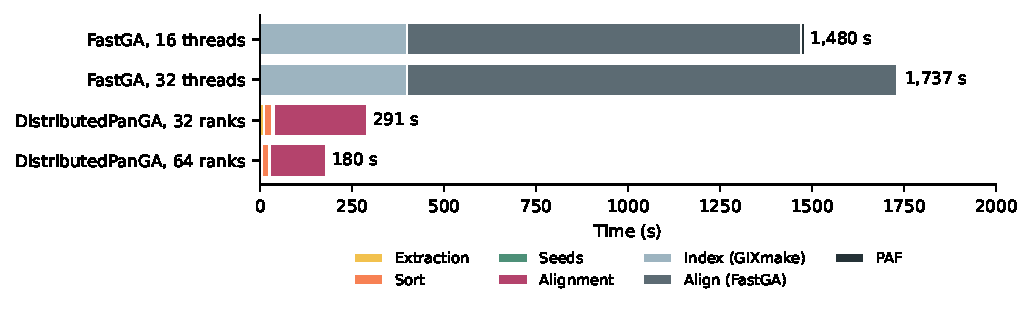
\includegraphics[width=\textwidth]{fig/human_chr6.pdf}
\caption{hsapiens90.chr6: time per stage for FastGA on one node and
DistributedPanGA on four nodes (Table~\ref{tab:human}).}\label{fig:human}
\par\noindent Alt text: Horizontal stacked bars. FastGA takes about 1,480
and 1,737 seconds, mostly alignment plus a 400-second index build;
DistributedPanGA takes about 291 and 180 seconds, mostly alignment.
\end{figure}
